\section{Brief history of particle physics}
Knowledge is a human need. For thousands of years we have been trying to understand the secrets of the universe. Such riddles fascinated even Johann Wolfgang von Goethe, as he wrote in his book Faust chapter 4 \cite{goethe1921faust} ; eine Tragedie, "What holds the world together in its innermost." 
Almost 400 years before Christ, an ancient Greek philosopher, Democritus, and his teacher Leukipp claimed that matter cannot be divided at will. Rather, there must be an Atomos (Greek: indivisible) that could no longer be subdivided.
Democritus was of the opinion that there were infinitely many atoms with different geometric forms that were in contact in a certain way. He pointed out that a thing has a color, taste or even soul, based on the apparent effect of the composition of these small grains.
\cite{capelle1968vorsokratiker}

This statement of Democritus was first laughed at by the renowned philosopher aristotiles. It took about 2000 years for a chemist named John Dalton to deal with the subject. Based on various test series, he summarized his conclusion in his book A New System of Chemical Philosophy, that all substances consist of spherical indivisible atoms. The atoms of different elements have different masses and volumes. This was exactly the most striking difference to Democritus's atomic world.\cite{dalton2010new}

The discovery of the periodic system by D. Mendeleev and P. Meyer enabled us to arrange the atoms according to their mass in such a way that their properties occur in a certain order.\cite{haken2013atom}

In 1897 Joseph Thompson was able to obtain a stream of particles by heating metals and deflecting them by a magnetic field. This electron beam was 200 times lighter than the lightest atom, hydrogen.
His conclusion was that atoms cannot be indivisible. He suggested that each atom consists of an electrically positively charged sphere in which electrically negatively charged electrons are stored - like raisins in a cake.

furthermore, renowned scientists as well as Marie and Pierre Curie have contributed much to the development of atomic theory by discovering radioactivity, Boltzmann by kinetic gas theory and M. Plank, the founder of quantum physics.
However, one of the most important steps in the atomic model was taken by the British physicist E. Rutherford. He bombarded a thin aluminium foil with a radioactive sample. If Thompson's cake model were correct, only a few alpha particles would be detected behind the aluminium foil. Surprisingly, many particles were visible, which could only be explained by the assumption that the majority of atoms consisted of empty spaces. Another miracle was that some particles could be seen above or below the target sample. Since we knew that the alpha particles were positively charged, we could assume the electric repulsive force of two positive charges. In 1911, RUTHERFORD created the planetary model of the atom, which was developed a year later by his pupil NIELS BOHR (1885-1962) into a model known as the Bohr atom model.
At first, however, it remained unclear what this core should consist of. \cite{haken2013atom, demtroder2005experimentalphysik}   
In 1912, the Austrian physicist Victor Hess discovered during his balloon flights that the ionization rate of the Earth's atmosphere increases with altitude. This result was not expected because until then the Earth's radioactivity was known as the only source of air ionization. Therefore, he postulated this new type of radiation as cosmic radiation, which must originate outside the Earth's atmosphere ~\cite{Ender}.\\
Further investigations two years later confirmed the thesis of a cosmic background of such radiation. After this new discovery, it was discovered that the radiation consists of charged particles. In 1932, the American physicist Carl David Anderson was able to prove the postulated particle of Dirac, the positron, as a component of an air shower through his cloud chamber. For a long time, cosmic rays were the only way to analyse such exotic particles.\cite{Bluemer:2009zf}
This changed when particle accelerators were able to generate particles in collisions. But even today, cosmic rays are the only way to study particles of the highest energies, since these energies cannot be reached by today's particle accelerators, such as the LHC. The LHC, the world's largest accelerator at CERN, produces particles with centre-of-mass energy equivalent to a cosmic particle of nearly $10^{17} eV $, with the energy spectrum of cosmic particles reaching up to $10^{20} eV $.
However, we can only analyse such exotic particles in detail by increasing the luminosity and procession of the particle accelerators at the nucleus. 
The discovery of the neutron by Chadwick (1932) showed that atomic nuclei are made up of protons and neutrons. It was also clear that, in addition to gravitation and the electromagnetic force,there should exist two short-range forces in nature: a strong force which binds the nucleons together and a weak force which is responsible for radioactive.
In the meantime it was agreed that a new theory was needed for the classification and grouping of this particle zoo. This is how the current standard model came into being.
The SLAC experiments showed that the electrons were scattering quasi-free point-like constituents inside the proton which were
soon identified with quarks. This was the first time that quarks
were shown to be dynamical entities, instead of bookkeeping devices to classify the hadrons (Gell-Mann’s eightfold way). \cite{griffiths2008introduction}
\section{Standard model}
The Standard Model in particle physics encompasses all of the
Elementary particles and their interactions. It is a gauge theory spontaneously broken by the Higgs mechanism with the gauge group $ SU(3)_C \otimes SU(2)_L \otimes U(1)_Y $.\\
From a theoretical point of view, the Standard Model is a quantum field theory that is based on local calibration invariance and consists of two rough parts. The electroweak sector $ SU(2)_L \otimes U(1)_Y $ is called GWS (\textbf{Glashow-Weinberg-Salam}) theory and describes the gauge bosons $ W^{\pm}, Z^0, \gamma $, the Higgs sector and its interaction with the leptons and quarks. In contrast to the other gauge bosons, the exchange particles of the weak interaction carry mass, which also affects the properties of the interactions. The color-charged sector $ SU(3)_C $, the chromo dynamics, deals with quarks and contains the eight massless, electrically neutral gluons gluons as gauge bosons. The gauge groups $SU(3)_C$ and $SU(2)_L$ are non-Abel gauge theories, more precisely Yang Mills theories.
A nice overview of the particle families with their respective exchange forces can be observed in the table below. 
The matter particles, fermions, will be divided into two large groups, leptons and quarks. Each group is arranged in 3 generations. Within the leptons there are three electrically neutral neutrionos families. The mass of the particles increases from generation to generation. Neutrinos only interact at the weak part, whereas the charged leptons interact both weakly and electromagnetically. Quarks are characterized by the fact that they can also interact strongly. They carry a charge of 2/3 or -1/3 and their mass increases from generation to generation. It should be particularly mentioned that the top quark with a mass of 173 GeV is by far the heaviest quark. The interaction between these fermions is based, as already mentioned, on the exchange of Bosons:



\section{Quantum chromo dynamics}

Nowadays, we know there are four types of interactions, see below:\\


\begin{tabular}{|c|c|c|c|c|}
\hline 
Interaction & Energy scale & Range [m] & Mediators \\ 
\hline 
Strong & $ \sim 1 $  & $10^{-15} $ & $g$ \\ 
\hline 
Electromagnetic & $ \sim 10^{-2} $ & $\infty$ & $\gamma $ \\ 
\hline  
Weak & $ \sim 10^{-6} $ & $10^{-18}$ & $W^{\pm}, Z$ \\ 
\hline
Gravity & $ \sim 10^{-38} $ & $\infty$ & maybe graviton \\ 
\hline 
\end{tabular}  
\\
\\
\\
Otherwise, it's clear meanwhile that nucleons are made up of quark and gluons.
Whereby, the gluons are the exchange bosons for this short interaction.
\begin{figure}[h!]
\centering
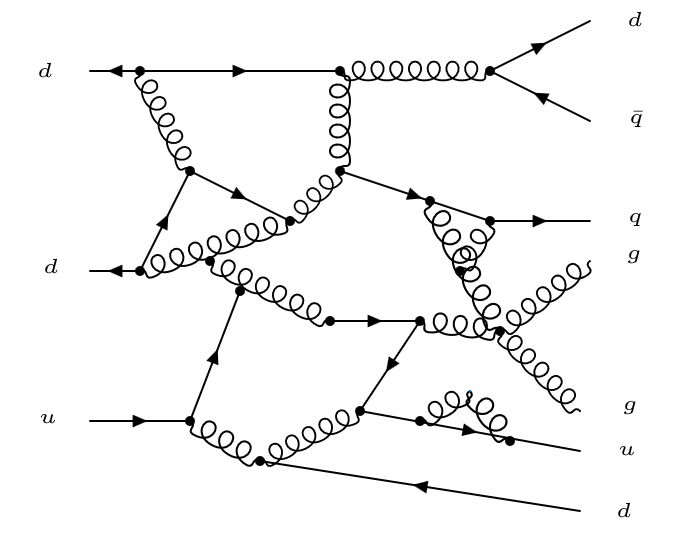
\includegraphics[scale=0.7]{images/Intro/Neutron.png}
\caption{That's a schematic picture of neutron structure. at the left side of the diagram is the low-resolution to see. The 3 quarks picture allows us to interpretate the quantum numbers of the neutron in the valence band.
We also obtain a high-resolution picture for a large $ Q^2 $. Here we have a lot of gluons (gluon sea) and quarks pair. \cite{Cunha13} \\ 
The interesting thing is, it doesn't matter in which energy scale we observe the quantum number of a neutron, because it is always the same.}
\end{figure}
To explain the short range of strong interaction Yukawa (1934) postulated mesons as a mediator for this force by the exchange of this massive field quanta. Three years later a candidate ($ \pi $ meson) was found in cosmic rays. Later on it was shown that Massive gauge field quanta break the gauge symmetry though so that the mediator must consequently be massless. But if they are based on the SU(3) gauge symmetry of the QCD\footnote{The quantum field theory which describes this area is called Quantum chromo dynamics short QCD.} Lagrangian massless how can the strong sector be short range? Another question came from a series experiments at SLAC. Through high-energy electron-proton scattering could make evidence of existence of quarks and their behaviour like free particles despite the energetically bound inner proton. The solution to these question was explained by Gross, Politzer
and Wilczek through asymptotic freedom. 
This effect can be proved by the running coupling and anti screening in QCD.
For the calculation the propagator loop correction in QCD we have to consider both quark loops (negative contribution $ \rightarrow $ screening) and gluon loops (positive contribution $ \rightarrow $ anti screening). 
\begin{figure}[h!]
\centering
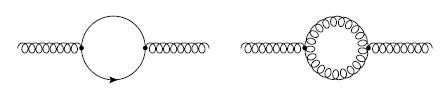
\includegraphics[scale=0.7]{images/Intro/quarkGluonPop.png}
\caption{Running coupling compared for QED, with a positive and QCD with a negative beta function}
\end{figure}

The one loop running coupling in QCD is:
\begin{equation}
\begin{split}
\alpha_s(Q^2)= \frac{\alpha_s(\mu^2)}{1+\beta_0 \alpha_s(\mu^2) ln(\frac{Q^2}{\mu^2})}
\end{split}
\end{equation}

Where $ \beta_0 = \dfrac{11N_c -2n_f}{12\pi} $, $ n_f $ comes from the first diagram and causes screening.  $ n_f $ is the number of quarks and $ N_c $ the number of colours and comes from the second diagram (anti screening). \\
Obviously, with $ n_f = 6 $ and $ N_c = 3 $ in standard model we will get $ \beta_0 >0 $. The Beta function is defined as:
\begin{equation}
\begin{split}
\beta(\alpha)=-(\beta_0 \alpha^2 + \beta_1 \alpha^3+\beta_2\alpha^4+....)=\frac{d\:\alpha(Q^2)}{d \:ln(Q^2)}
\end{split}
\end{equation}

e.g. $ -(\beta_0 \alpha^2) <0 $ will be negative, which is actually the opposite of QED with $ \beta_0=- \dfrac{\pi}{3} \rightarrow -(\beta_0 \alpha^2) >0 $ ! That means coupling constant in QCD will increase
with decreasing $ Q^2 $ (increasing distance), In QED vice versa.
\begin{figure}[h!]
\centering
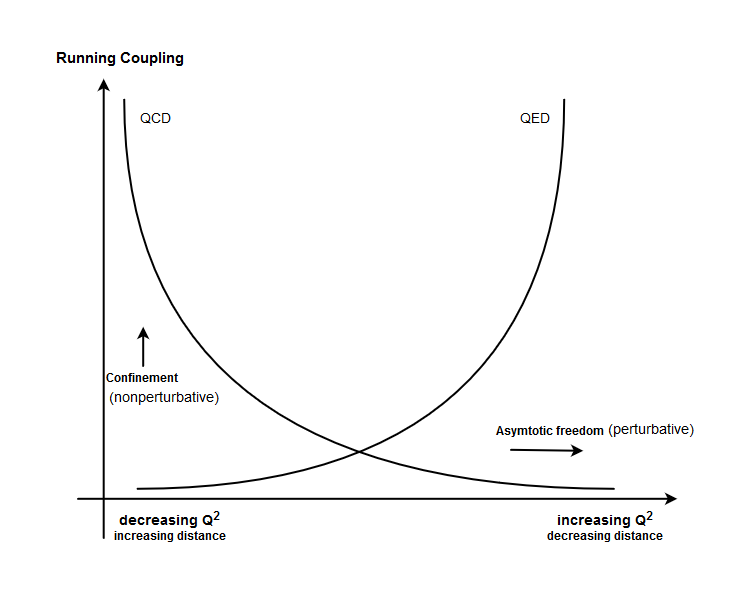
\includegraphics[scale=0.7]{images/Intro/QCDRunningCoupling.png}
\end{figure}



Asymptotic freedom allows us to use perturbation theory \footnote{Actually there is need of two more things, if we want to make the connection between theory and experiment: either infrared safety or factorisation. That will be discussed in the next chapter}.
Quarks have not yet been observed as free particles. With increasing separation it will be easier to produce quark-antiquark pair than to isolate quark because the coupling between them too strong is. This mechanism is called confinement. Confinement It has been confirmed in Lattice QCD, but not yet mathematically. It belongs to  nonperturbative theory.
Quarks prefer to bind into hadrons what can be classified to baryons with three quarks state and mesons with a quark-antiquark state.
As we know, the wave function of fermions must be antisymmetric according to Pauli exclusion principle under the exchange of two quarks. Interestingly, there are resonance states with spin $ \frac{3}{2} $ like $ {\Delta}^{++} $.
The spins of the three up quarks are parallel to each other, have the same flavour and orbital angular momentum L=0. This means that an exchange of flavour, spin and space (orbital angular momentum) does not lead to any change. This problem is solved with the additional degree of freedom, the so-called color charge. Each quark comes in one of three colours red, green or blue and also anticolour $ \bar{r}, \bar{b}, \bar{g} $ for antiquarks. The hadrons are colour singlets in regard with the hypothesis,
, they are invariant under rotations in colour space. The colour hypothesis describes the existence of mesons with $ q \bar{q} $ and baryons with $ qqq $. because if the wave function is odd in color, we have solved the spin statistical problem.
The total wave function for each particle can be expressed in terms of:

\begin{equation}
\begin{split}
\Psi_{3q} &= \psi_{space} \times \chi_{spin} \times \theta_{colour} \times \phi_{flavour} \\
&\:\:\:\:\:\:\:O(3) \:\:\:\:\: SU(2)\:\:\:\: SU(3)\:\:\:\:\: SU(6)\\
\end{split}
\end{equation}
Now we can compute all possible States in regard to colour With Young Tableaux \cite{Greiner1989}. One uses group theory methods, for instance the Young Tableaux technique, to decompose products of irreducible representations into sums.
\begin{figure}[h!]
\centering
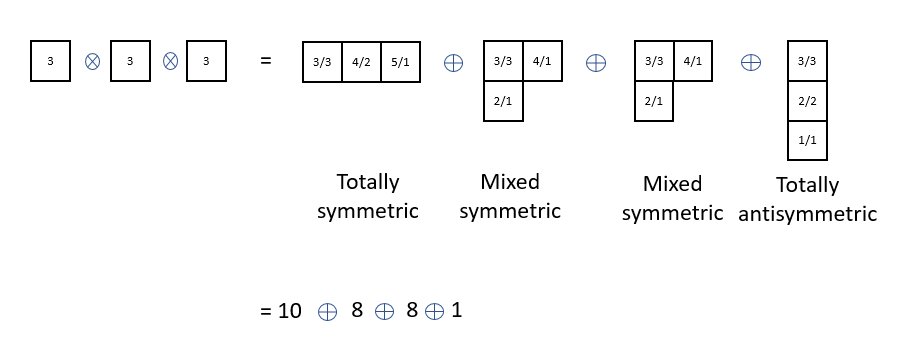
\includegraphics[scale=0.7]{images/Intro/Young.png}
\end{figure}

After using The same procedure for SU(2) and SU(6) for spins and flavours of the three quarks we will get:

\begin{equation}
\begin{split}
2\: \otimes\:2 \:\otimes\:2 &= 4 \:\:\:\oplus\: 2\:\:\:\oplus\:2\:\:\:\oplus\:0\\
6\: \otimes\:6 \:\otimes\:6&= 56 \:\oplus\: 70\:\oplus\:70\:\oplus\:20
\end{split}
\end{equation}

As we can see, the total wave function is most complicated in the QCD area. That's the reason why the Lagrangian of QCD is always given in the short form. I'll get to the bottom of Lagrangian in QCD later. 
Before the QCD is formulated as a gauge theory, an experiment should be pointed out which makes clear why there is an additional degree of freedom in the QCD and why there is no
U(1)-symmetry here. Looking at the electron-positron scattering again, it is important to realize that not only $ \mu^+ \mu^- $, but also $ e^+ e^- $,$ \tau^+ \tau^- $ and also $ q \bar{q} $ can arise, where the quark pairs fragment into hadrons. For the ratio:
\begin{equation}
\begin{split}
R = \frac{\sigma(e^+e^- \rightarrow Hadronnen)}{\sigma(e^+e^- \rightarrow \mu^+ \mu^-)}
\end{split}
\end{equation}

one would expect, due to the fact that the coupling takes place over the charge, that only the sum over the square of the quark charges (because $  {e^2}_\mu= 1$) contributes. However, there is an additional factor $N_C$ that can be determined experimentally
\begin{equation}
\begin{split}
R = N_C \sum_q e^2_q
\end{split}
\end{equation}
Without this factor one would expect for $ u, d, s $, $ u, d, s, c $ and $ u, d, s, c, b $ Respectively $ \frac{2}{3}, \frac{10}{9}, \frac{11}{10} $ The experiment showed a third of the respective results though (i.e. $ N_C =3 $):

\begin{figure}[h!]
\centering
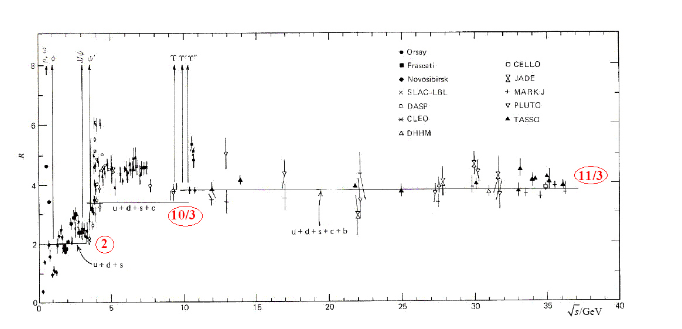
\includegraphics[scale=0.6]{images/Intro/Ratio.png}
\cite{Eva}
\end{figure}
\section{QCD Lagrangian}

QCD like QED and the weak interaction theory is described by representations of a symmetry group. From the condition that the Lagrangian must be invariant under arbitrary global and local symmetry transformations (Noether’s theorem) follows the interactions terms.
The Lagrangian of QCD is invariant under $ U(3) = U(1) \times SU(3) $ global trafo. I'm just going to look into $ SU(3) $. We can replace the three Pauli matrices from $ SU(2) $ in the Yang-Mills theory by the eight Gell-Mann matrices $ {\lambda}^a $ with following relation:
\begin{equation}
\begin{split}
&T^a = \frac{1}{2} \lambda^a\\
&[T^a, T^b]= if^{abc} T^c \:\:\:\:\:\:\:\:\:\:\:\:\:\:\text{fundamental representation}\\
&({T^a}_{adj})_bc = -if^{abc} \:\:\:\:\:\:\:\:\:\:\:\:\text{adjoint representation}
\end{split}
\end{equation}
To quantize QCD theory is usually used the Faddeev-Popov in the path integral to fix a gauge and define a gluon propagator. The Lagrangian is given:

%L. D. Faddeev and V. N. Popov, \Feynman diagrams for the Yang-Mills eld", Phys. Lett.
%B 25, 29 (1967).
\begin{equation}
\begin{split}
& \mathscr{L} = \mathscr{L}_{free}+{\color[RGB]{255,0,0} \mathscr{L}_{int}}\\
& \mathscr{L} = \sum_f \bar{\psi}_{if} (i\gamma^{\mu} {\partial}_{\mu}-m_f){\psi}^{if}-\frac{1}{4}{F_a}^{\mu \nu}{F^a}_{\mu \nu}-\frac{1}{2\xi}(\partial^{\mu} {A^a}_{\mu})(\partial^{\nu} {A^a}_{\nu})+(\partial^{\mu} {\chi^a}^*)(\partial_{\mu} {\chi^a})\\
&{\color[RGB]{255,0,0} -g_s \bar{\psi}_{i} {T^a}_{ij}{\psi}_{j} \gamma^{\mu} {A^a}_{\mu}-\frac{g_s}{2} f^{abc}(\partial_{\mu} {A^a}_{\nu}-\partial_{nu} {A^a}_{\mu}{A_b}^{\mu}{A_c}^{\nu})-\frac{{g_s}^2}{4} f^{abc} ({A_b}^{\mu}{A_c}^{\nu}f^{ade} ({A^d}_{\mu} {A^e}_{\nu})}\\
&{\color[RGB]{255,0,0} -g_s f^{abc} (\partial^{\mu} {\chi^a}^{*}){\chi^b}{A^c}_{\mu}}\\
\end{split}
\end{equation}

Here i,j are color indices in the fundamental representation, a  color index in the adjoint representation of SU(3) respectively. f labels the six flavours of quarks. $ g_s $ describes the strong coupling constant and $ {A^a}_{\mu} $ is the gluon field and it corresponds to anon-abelian gauge theory with structure constants $ f^{abc} $. $ {\chi^a} $ is a scalar field under Lorenz group, but anti commuting. With The field-strength tensor for QCD by \cite{Schwartz:2013pla, peskin2018introduction}
\begin{equation}
\begin{split}
{F^a}_{\mu \nu}= \partial_\mu {A^a}_{\nu}-\partial_\nu {A^a}_{\mu}-g_s f_{abc} {A^b}_{\mu} {A^c}_{\nu}
\end{split}
\end{equation}

\begin{figure}[h!]
\hspace{-1cm}
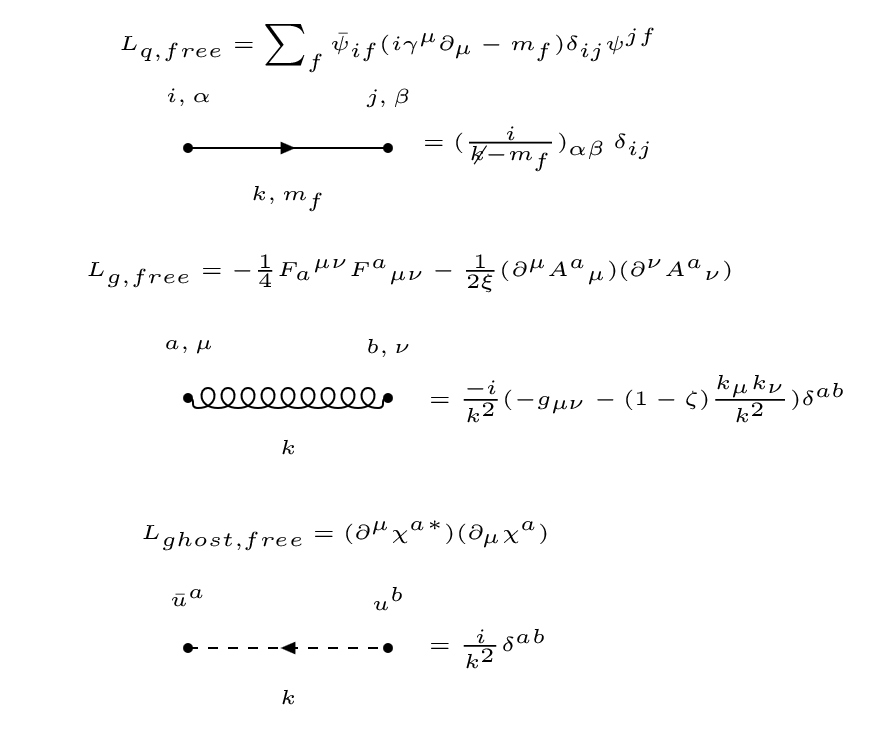
\includegraphics[scale=0.5]{images/Intro/Lfree.png}
\end{figure}


It can be shown that the above Lagrangian is invariant under the following $ SU(3) $ gauge transformations:
\begin{equation}
\begin{split}
&{\psi}^{\prime}(x) \rightarrow exp(i \:\eta_a(x) \:T^a) \:\psi(x)\\
&{D}^{\prime} \rightarrow \partial_\mu+ig_sT_a\: {{A}^{\prime}}^a_{\mu } \\
&{{A}^{\prime}}^a_{\mu }\rightarrow  {A^a}_{\mu}- \frac{1}{g_s}\partial_\mu \eta^a(x)+ f^{abc} \eta_{b}(x) {A_c}_{\nu}(x)
\end{split}
\end{equation}

\newpage
\section{Colour factor calculation}
In this section we will calculate the Casimir operators of the respective diagrams for later goals.
Fundamental representation in $ SU(3) $ are given by\cite{Schwartz:2013pla, Platzer:2018pmd}
\begin{equation}
\begin{split}
T^a = \vartheta^a \equiv \frac{\lambda ^2}{2} \:\:\:\:\:\:\: \mathit{with\: Gell-Mann\: matrices\: \lambda ^a}
\end{split}
\end{equation}

\begin{equation}
\begin{split}
\lambda ^1 =\begin{pmatrix} 0& 1 &\\ 1& 0 &\\ & & 0 \end{pmatrix},\:\:\: \lambda ^2 =\begin{pmatrix} 0& -i &\\ i& 0 &\\ & & 0 \end{pmatrix}, 
\:\:\: \lambda ^3 =\begin{pmatrix} 1&  &\\ & -1 &\\ & & 0 \end{pmatrix}, \:\:\: \lambda ^4 =\begin{pmatrix} &  &1\\ & 0&\\1 & &  \end{pmatrix}\\\
\lambda ^5 =\begin{pmatrix} &  &-i\\ & 0 &\\ i& &  \end{pmatrix},\:\:\: \lambda ^6 =\begin{pmatrix} 0&  &\\ & 0 &1\\ & 1& 0 \end{pmatrix}, 
\:\:\: \lambda ^7 =\begin{pmatrix} 0&  &\\ & 0 &-i\\ & i& 0 \end{pmatrix}, \:\:\: \lambda ^8 =\frac{1}{\sqrt3}\begin{pmatrix} 1&  &\\ & 1&\\ & &-2  \end{pmatrix}
\end{split}
\end{equation}
As we can see, $ {\lambda}^3 $ and $  {\lambda}^8 $ are diagonal.
These generators satisfy:\\ 
\\
\begin{figure}[h!]
\centering
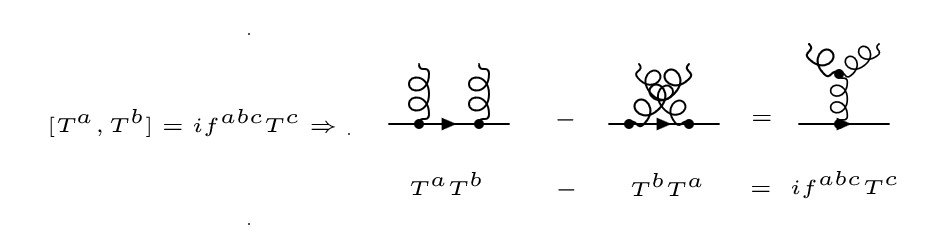
\includegraphics[scale=0.6]{images/Intro/Casimir.png}
\end{figure}
Or in the adjoint representation:\\
\\
\begin{figure}[h!]
\centering
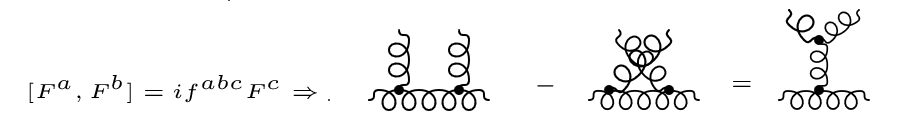
\includegraphics[scale=0.6]{images/Intro/CasimirAdj.png}
\end{figure}

The most common convention for the normalization of the generators in physics is:
\begin{equation}
\displaystyle\sum\limits_{c,d} f^{acd} f^{bcd} = N \delta^{ab}
\end{equation}
One of the most important equation for the colour factor calculation is the Jaccobi-Identity:
\begin{equation}
\begin{split}\:
[T^a, [T^b , T^c]]+[T^c, [T^a , T^b]]+[T^b, [T^c , T^a]]=0
\end{split}
\end{equation}
If we write this in terms of the structure constant, we'll get:
\begin{equation}
\begin{split}\:
f^{axd} f^{bcx} +  f^{cxd} f^{abx} +f^{bxd} f^{cax} =0
\end{split}
\end{equation}
So we are able to compute:
\begin{equation}
f^{abc} = -2i\: tr(T^a[T^b, T^c])
\end{equation}
generalize to:
\begin{equation}
f^{abc}f^{xcd} = 4i\: tr(T^a[T^b, [T^c, T^d]])
\end{equation}

With this relations we can calculate all Casimir operators:\\
\begin{figure}[h!]
\centering
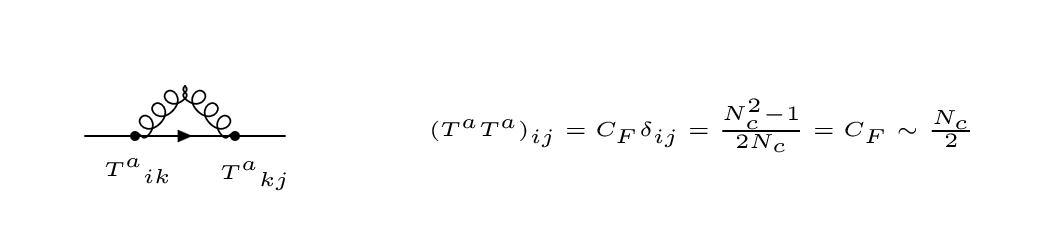
\includegraphics[scale=0.6]{images/Intro/Casimir1.png}
\end{figure}
\begin{figure}[h!]
\centering
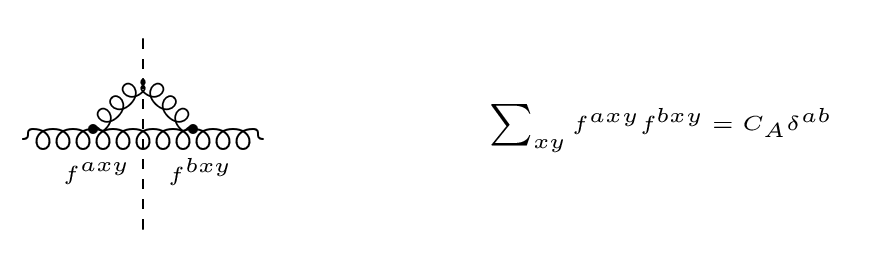
\includegraphics[scale=0.6]{images/Intro/Casimir2.png}
\end{figure}
\pagebreak
\\
Which means the charge of gluon is twice a quark because:
\begin{equation}
 C_A = N_c =2C_F \sim 2(\frac{N_C}{2}) 
\end{equation}
\begin{figure}[h!]
\centering
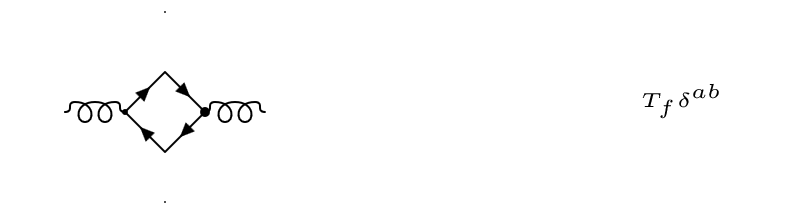
\includegraphics[scale=0.6]{images/Intro/Casimir3.png}
\end{figure}
\begin{figure}[h!]
\centering
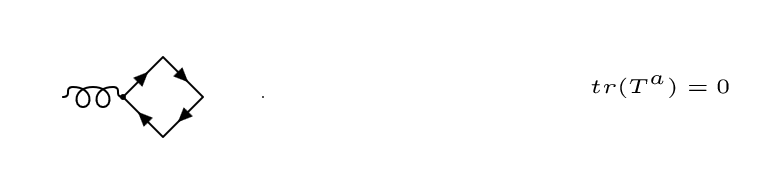
\includegraphics[scale=0.6]{images/Intro/Casimir4.png}
\end{figure}


One of the most important relation in this case is the Fierz identity. It shows the difference between QED and QCD!
\begin{equation}
\displaystyle\sum\limits_{a} {T_{ij}}^a {T_{kl}}^a = \frac{1}{2}(\delta_{il}\delta_{kj}-\frac{1}{N}\delta_{ij}\delta_{kl})
\end{equation}
Graphically it means:
\begin{figure}[h!]
\centering
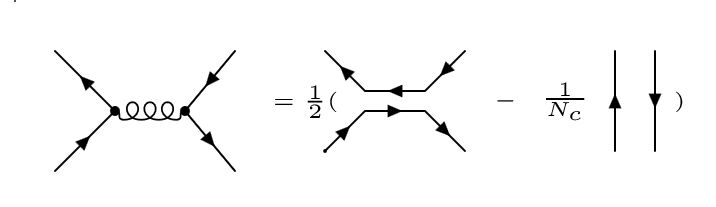
\includegraphics[scale=0.6]{images/Intro/Fritz.png}
\end{figure}
The charge transfer in QED takes place along the Fermion line because photons cannot transport charges. On the other hand, the gluons can transfer color charges because they have color charges themselves.  

The main relation we will use later for SU(N):
\begin{equation}
tr(T^a T^b)= {T_{ij}}^a {T_{ji}}^b = T_F \delta^{ab}
\end{equation}
\begin{equation}
\displaystyle\sum\limits_{a} (T^a T^a) = C_F \delta^{ij}
\end{equation}
\begin{equation}
f^{acd} f^{bcd} = C_A \delta^{ab}
\end{equation}
With $  T_F = \frac{1}{2} $ , $ C_A = N $ and $ C_F = \frac{N^2 -1}{2N} $.



\newpage